\subparagraph*{Submission : }
\textit{Consider the case in which prices are fixed, but the assignment of promos to users need to be optimized by using an assignment algorithm. All the parameters need to be learnt.}\\

The submission requires to learn the assignment of the promotions to the diffferent customer category. This time we are dealing with a matching problem. 

\subsection*{Basic knowledge}
DIRE CHE BANDIT PROBLEM è e RIVEDERE SE QUELLI PRECEDENTI SONO GIUSTI. AGGIUNGERE UN PO' DI TEORIA

A Matching Problem can be modeled as a graph $G=(N,A)$, where $N$ is a set of node and $A$ is a set of arc. A matching $M$ is a subset of $A$ such that each node is connected to at most one node with at most one arc of $M$. The problem can be seen as a maximization problem where the objective is to determine the matching of maximum cardinality.\\

\subparagraph*{UCB Matching}
We can design a bandit algorithom that solve the mathing problem. A classical UCB approach is combined with a linear sum assignement algorithm, a well known algorithm that given a bipartite graph solve the matching problem. The learner will retrieve a the subset of arc that correspond to the optimal matching. 
At $t$, play a superarm $a_{t}$ such that:\\
$a_{t} \leftarrow \argmax\limits_{\textbf{a} \in M}{\left\{\sum\limits_{a \in \textbf{a}}\bar{x}_{a,t} + \sqrt{\frac{2 log(t)}{{n_{a}(t-1)}} }\right\}}$ \\
where $M$ is the set of matches.

\subparagraph*{Promo-Category UCB Matching}

We have slightly modifying the previously implemented UCB Matching. \\
We introduce two matrixes, with the same shape of the promotion-category graph, used for the maximization problem, representing the matching between a specific customer category and a specific promo. The first matrix represent the total collected rewards for that specific assignement, the second is used as support and contains the number of occurences that the assignement has been chosen (a customer of that category to which it was proposed the second item with that promo). 
Those matrix are updated by the reward obtained by the currently served customer and used to calculate the average reward of each possible assignment. The average value are used to feed the default UCB Matching learner in order to update the confidence bound.
An initialization phase is needed in order to explore and learn the average reward for all the possible configurations. For this reason we introduce a staring dalay in which we explore all possible configurations in an exaustive way and store the rewards. In this phase the learner do not compute the optimal solution for the matching problem, but retrieves a known matching that change at each iteration.
As for the other learners, the rewards are normalized dividing the actual reward by the maximum possible reward.

\subsection*{Strategy}

As always we simulate the randomly arrival of the customers and the purchase at a fixed price of the first item. In case the customer purchase the \textit{Racing Skis}, we ask to the learner (our custom UCB matching learner) to retrieve the optimas assignemnt promotions-category. According to the user category, and the pulled assignment promo-category, we compute the discounted price for the second item and we propose it to the customer. In important to note that the learner provides us a set of arms, but we use only the assignement that involve the category of the currently served user. The user reward is calculated as the sum of the reward obtained by the sold of the first item plus the eventually sold of the sencond. However, since our goal it to lorne the matching for the fromo-category of the second item, and the price of the \textit{Racing Skis} is fixed, we feed the matching learner with the reward obtained by the sold of the \textit{Racing Ski Helmet}. 

\subparagraph{Implementation} 
\begin{itemize}
	\item No seasonality, conversion rate do no change
	\item Price of the \textit{Racing Skis} is fixed to 1980.0
	\item Conversion rate associated with the first item is not known
	\item Basic price of the \textit{Racing Ski Helmet} is fixed to 630.0
	\item Conversion rate associated with the second item is not known
	\item Optimal promotion-category assignment need to be learnt
\end{itemize}

\subparagraph{Optimal strategy}The optimal strategy, used to compute the regret, is calculated in an offline manner, calculating for each possible promotion-category the expected reward, obtained multiplyng the conversion rate of the category with the discounted price. The obtained matrix of the expected rewards is then evaluated with a Linear Sum Assignement algorithm that maximize the total expected reward, retrieving the optimal assigment. The obtained optimal solution is:\\
\begin{center}
	\begin{tabular}{ |c|c|c|} 
	\hline
	User category & Assigned promotion & Racing Ski Helmet price \\
	\hline
	Sport Addicted & P$_2$ : 20\% & 504.0 \\
	\hline
	Gifter & P$_1$ : 10\% & 567.0 \\
	\hline
	Amateur & P$_0$ : 0\% & 630.0 \\
	\hline
	Worried & P$_3$ : 30\% & 441.0 \\
	\hline
	\end{tabular}
\end{center}

\subsection*{Results}
\begin{center}
	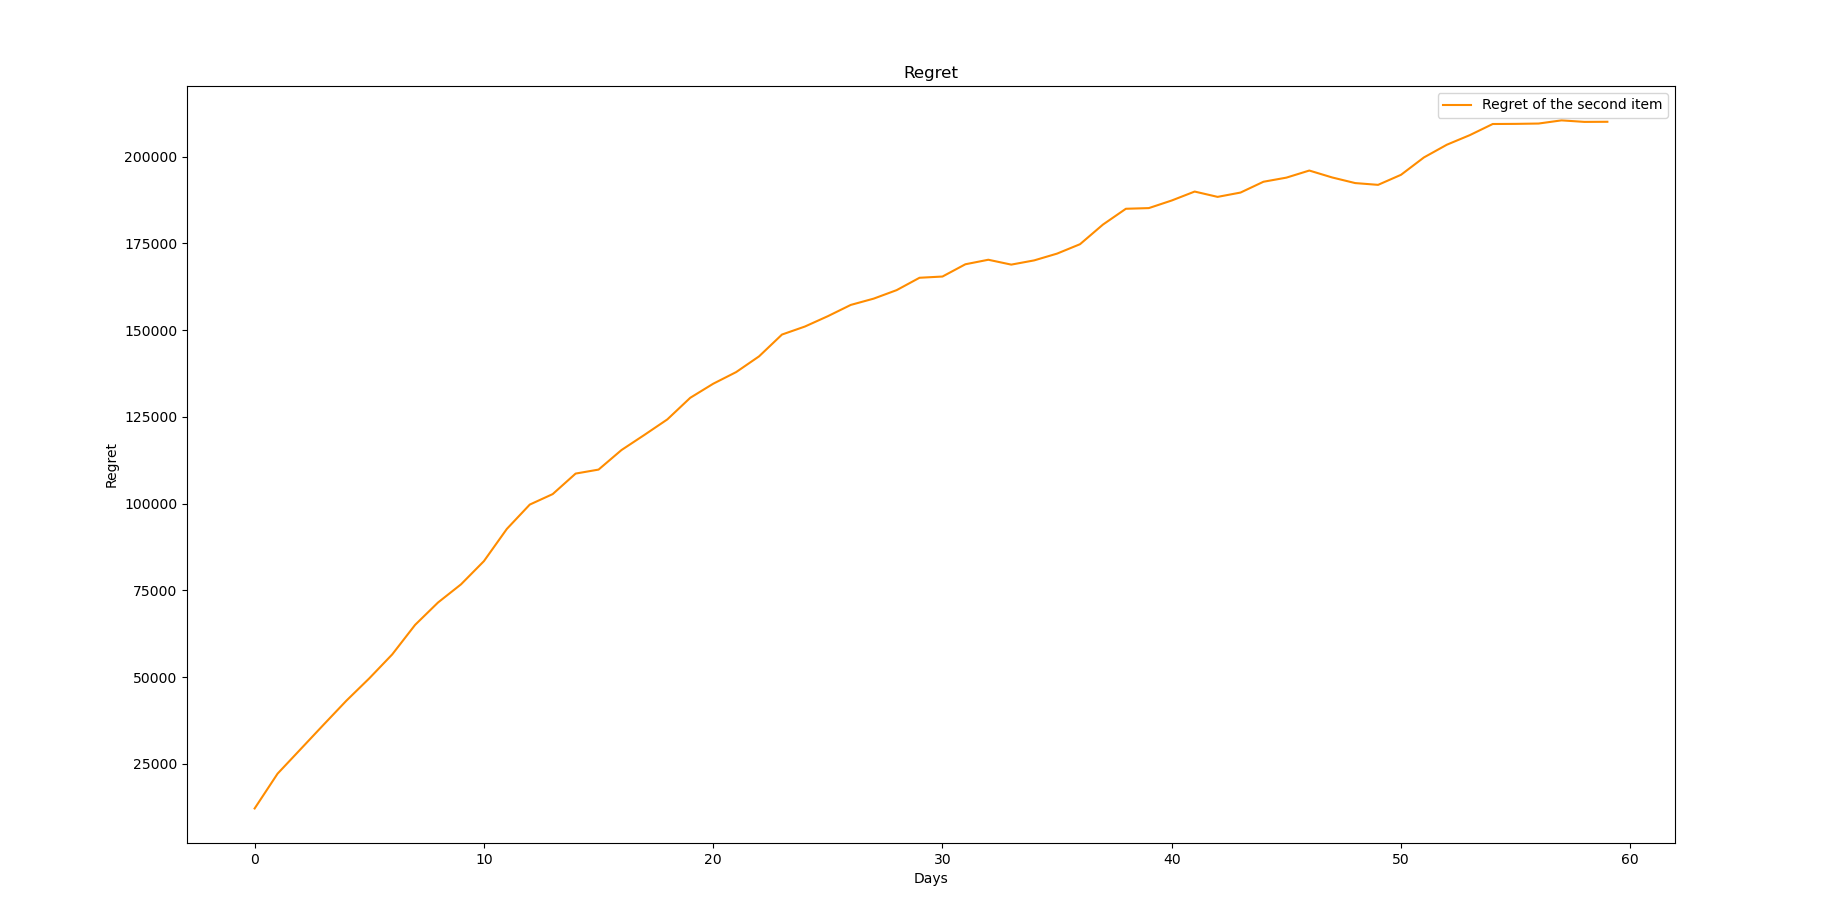
\includegraphics[scale=0.30]{Images/n5}
\end{center}
Days: 60\\
Experiments number: 5 \\
Starting delay of the Promo-Category UCB Matching: 1000 clients\\
UCB Matching at the end converge to the optimal solution \\
\subsection*{Considerations}
We can observe that the UCB Matching algorithm has a linear increase on the cumulative regret for the first thirty days, but after that, it becomes more and more stable on the optimal matching, and the cumulative regret does not increase so much.